\documentclass[11pt]{article}
\usepackage{geometry}                
\geometry{letterpaper}                   

\usepackage{graphicx}
\usepackage{amssymb}
\usepackage{epstopdf}
\usepackage{natbib}
\usepackage{amssymb, amsmath}
\DeclareGraphicsRule{.tif}{png}{.png}{`convert #1 `dirname #1`/`basename #1 .tif`.png}

%\title{Intersection Problem}
%\author{Marcel Arikan, Nuhro Ego, Ralf Kohrt}
%\date{date} 

\begin{document}



\thispagestyle{empty}

\begin{center}
\includegraphics[width=5cm]{ETHlogo.eps}

\bigskip


\bigskip


\bigskip


\LARGE{ 	Lecture with Computer Exercises:\\ }
\LARGE{ Modelling and Simulating Social Systems with MATLAB\\}

\bigskip

\bigskip

\small{Project Report}\\

\bigskip

\bigskip

\bigskip

\bigskip


\begin{tabular}{|c|}
\hline
\\
\textbf{\LARGE{Intersection Problem}}\\
\textbf{\LARGE{Traffic flow comparison of roundabouts with crossroads}}\\
\textbf{\LARGE{controlled by trafficlights, including pedestrians}}\\
\\
\hline
\end{tabular}
\bigskip

\bigskip

\bigskip

\LARGE{Marcel Arikan, Nuhro Ego, Ralf Kohrt}



\bigskip

\bigskip

\bigskip

\bigskip

\bigskip

\bigskip

\bigskip

\bigskip

Zurich\\
Dec 2012\\

\end{center}



\newpage

%%%%%%%%%%%%%%%%%%%%%%%%%%%%%%%%%%%%%%%%%%%%%%%%%

\newpage
\section*{Agreement for free-download}
\bigskip


\bigskip


\large We hereby agree to make our source code for this project freely available for download from the web pages of the SOMS chair. Furthermore, we assure that all source code is written by ourselves and is not violating any copyright restrictions.

\begin{center}

\bigskip


\bigskip


\begin{tabular}{@{}p{3cm}@{}p{4cm}@{}@{}p{4cm}@{}@{}p{4cm}@{}}
\begin{minipage}{2cm}

\end{minipage}
&
\begin{minipage}{4cm}
\vspace{2mm} \large Marcel Arikan

 \vspace{\baselineskip}

\end{minipage}
&
\begin{minipage}{4cm}
\vspace{2mm} \large Nuhro Ego

 \vspace{\baselineskip}

\end{minipage}
&
\begin{minipage}{4cm}

\large Ralf Kohrt

\end{minipage}
\end{tabular}


\end{center}
\newpage

%%%%%%%%%%%%%%%%%%%%%%%%%%%%%%%%%%%%%%%



% IMPORTANT
% you MUST include the ETH declaration of originality here; it is available for download on the course website or at http://www.ethz.ch/faculty/exams/plagiarism/index_EN; it can be printed as pdf and should be filled out in handwriting


%%%%%%%%%% Table of content %%%%%%%%%%%%%%%%%

\tableofcontents

\newpage

%%%%%%%%%%%%%%%%%%%%%%%%%%%%%%%%%%%%%%%



\section{Abstract}

\section{Individual contributions}

\section{Introduction and Motivations}

\section{Description of the Model and Implementation}

\subsection{Description of the main loop}

In our model one can compare roundabouts with crossroads, controlled by traffic lights (which we will call \texttt{crosslight}), with each other. One can use an arbitrary combination of roundabouts and crosslights in a $N \times M$ map. \\
The simulation can be done with different probabilities for the car to go straight and left and right will have the same probability but depend on the probability ahead. One can also choose different car and pedestrian densities. 
The simulation will generate a plot over these densities as x- and y- axis and the average flow $flow = density \cdot speed$ and average speed as z-axis. 

\subsubsection{Implementation}

We have a big matrix which shows all roads and intersections. And many smaller ones, 2 for every lane, which contain all the lanes for every road after each other. 
The first one contains the positions of the cars and the second one contains their speed. And one for every array which is used by a \texttt{crosslight} or roundabout intersection and needs to be stored for calculating the next step.\\

For almost every one of those arrays we have to arrays, one for the current state which is shown on the screen and one for the next step which contains the next step, which will be calculated cell for cell. 
After the calculation the next step will be stored in the first array and the calculation starts over again.

\subsection{Roundabout}
Our implementation of the roundabout consits of a circle with 12 cells and 4 roads, which lead towars it. Every street has pedestrian crossings in front of each roundabout. 
Like in the real world, cars inside the roundabout have priority over cars wanting to enter them and pedestrians have priorithy over cars at the pedestrian crossings, 
with the addition, that pedestrians will only walk on the road if there is no car staying or driving on the cell they wants to walk on. 
Inside the crossroad the speed a car can have is limited to 1 cell per iteration. \\

A car which wants to leave the roundabout at the next exit will indicate, in our plot this is shown by giving these cars a darker colour. 
The exit a car will take is calculated from the probability ahead like in the crossroad, but with a fixed probability of 5 \% for a car which will take the 4th exit (i.e. the car will turn around). \\
\subsubsection{Implementation}
This is implemented with many arrays, three arrays for the circle, one which shows whether there is a car or not and if the car wants to leave at the next exit. 
The second is used to store the velocity of the car and the third is used to store how many exits the car will pass without leaving.\\

For the pedestrians we use a yellow colour on the street (a car is blue), and two 'buckets' between the lanes of each road so that they will cross both lanes of a road.


\section{Simulation Results and Discussion}

\section{Summary and Outlook}

\section{References}






\end{document}  



 
